\chapter{Data Set}
\label{chapter:hps:dataset}

Proper search for \ac{dm} signals within the \ac{hps} detector includes both collection of data
with the \ac{hps} detetor and simulation of how this apparatus responds to the physics of specific
processes. This chapter is focused on detailing the origin of these samples. The collected data can
be characterized by the known inputs from \ac{cebaf} and the run time. The simulation, as one might
expect, is a complicated multi-stage procedure in order to appropriately reflect the intricacies of
the real data.

\section{Collected Data} \label{sec:hps:data}
The data used in this study was collected over a series of 82 data collection runs within 2016
yielding a total of \todo[lookup]{lookup how much total data was collected in 2016} days of
continuous beam. The full luminosity of this data is estimated to be $10.7~\text{pb}^{-1}$. As
alluded to in \cref{sec:hps-ecal}, the collected data was triggered in order to focus the sample on
specific data of interest. The specifics of this trigger are important for simulation as well as
understanding the accessibility of different models from this dataset. \todo[lookup]{details of
  2016 pair-wise trigger should be copied in for reference.}

\section{Simulation} \label{sec:hps:sim}
As mentioned the simulation goes through many steps in order to account for the different physics
processes that are of interest in a realistic fashion. In general, these steps are
\begin{enumerate}
  \item Generation -- using a tool like {\sc MadGraph/MadEvent}\todo[citation]{MG/ME citation} to generate
        specific events from Feynman diagrams
  \item Displacement -- if the sample expects to have the decay products be displaced (for example in the
        SIMP signal process), displace these decay products with a \emph{uniform} distribution of decay
        lengths to allow for re-weighting.
  \item Simulation -- simulate the detector response with \textsc{Geant4}\cite{geant4}
  \item Emulation -- emulate the readout electronics and triggering mechanism of collected data
\end{enumerate}
After this emulation stage, we can treat the simulation the same as the collected data,
applying the reconstruction and further analysis manipulatiuons and selections.

Moreover, simulated samples of standard data allows us to study how the detector responds in the
absence of such a signal process. These samples are produced in a similar way as iDM signal - just
with a different original generation step initializing the event (and inserting the physical
displacement distribution instead of a uniform one).

\section{Reconstruction}
\todo[lookup]{Brief overview of how events are reconstructed,
  especially with regard to tracks and vertices.}

\section{Analysis Pre-Selection}
The final stage that all events go through is a rudimentary pre-selection which simplifies the
resulting shape of the data in the event such that final analysis is not as complicated.
Specifically, the pre-selection for this analysis is requiring exactly one vertex to be
reconstructed within the event. This requirement naturally disposes of events which are cluttered
with particles from other beam arrivals (thus causing more than one vertex to be reconstructed) and
events which do not have a electron-positron pair within acceptance (thus causing no vertices to be
reconstructed). \cref{fig:n-vertex-pre-selection} shows the distribution of number of vertices
within an event for a variety of samples.

\begin{figure}
  \centering
  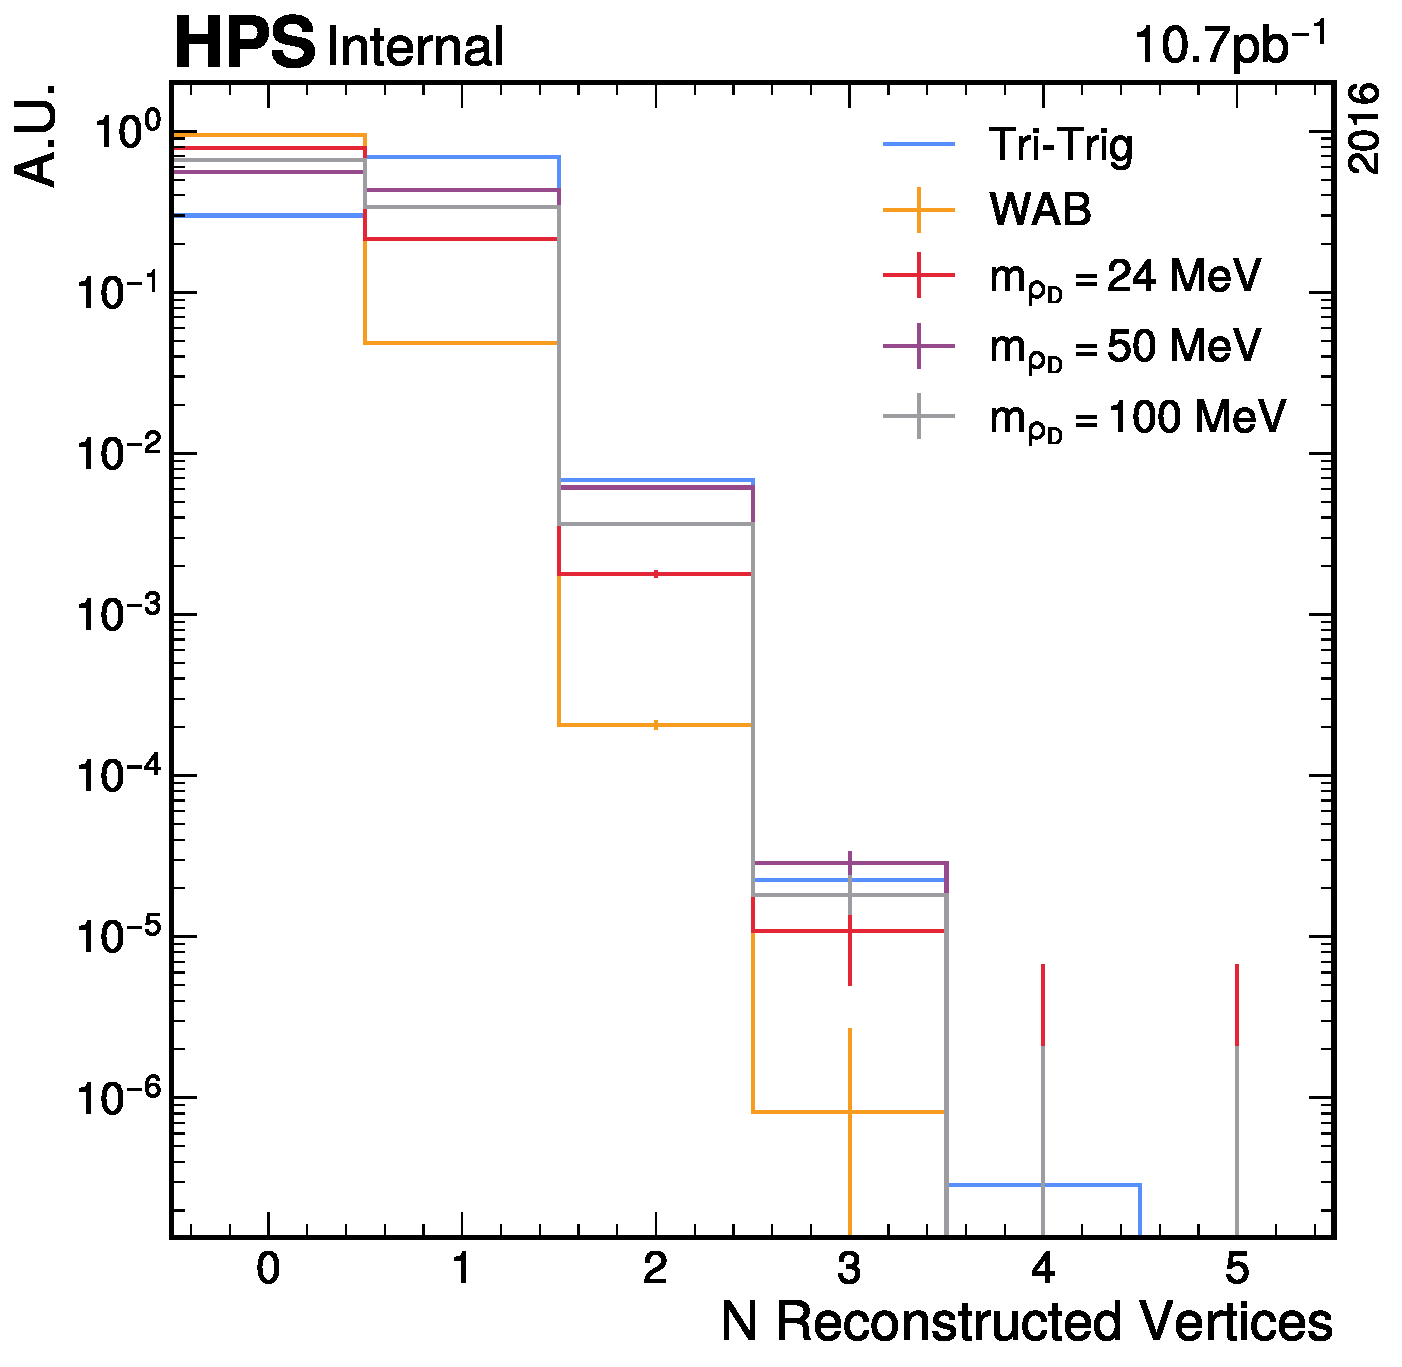
\includegraphics[width=0.5\textwidth]{figures/hps/dataset/n-vertex-pre-selection-mc-only.pdf}
  \caption{Number of vertices reconstructed within the simulation samples.}
  \label{fig:n-vertex-pre-selection}
\end{figure}